% !TeX program = xelatex*2
% !TeX root = ../elegantnote.tex
\section{绪论}
\subsection{误差的来源和分类}
\begin{definition}[舍入误差]
    由于计算机字长的有限性,对相关数据进行存储表示时便产生舍入误差。
\end{definition}
\begin{definition}[截断误差]
    计算机必须在有限的时间内得到运行结果,于是无穷的运算过程必须截断为有限过程,由此产生截断误差。
\end{definition}
\begin{figure}[htbp]
    \centering
    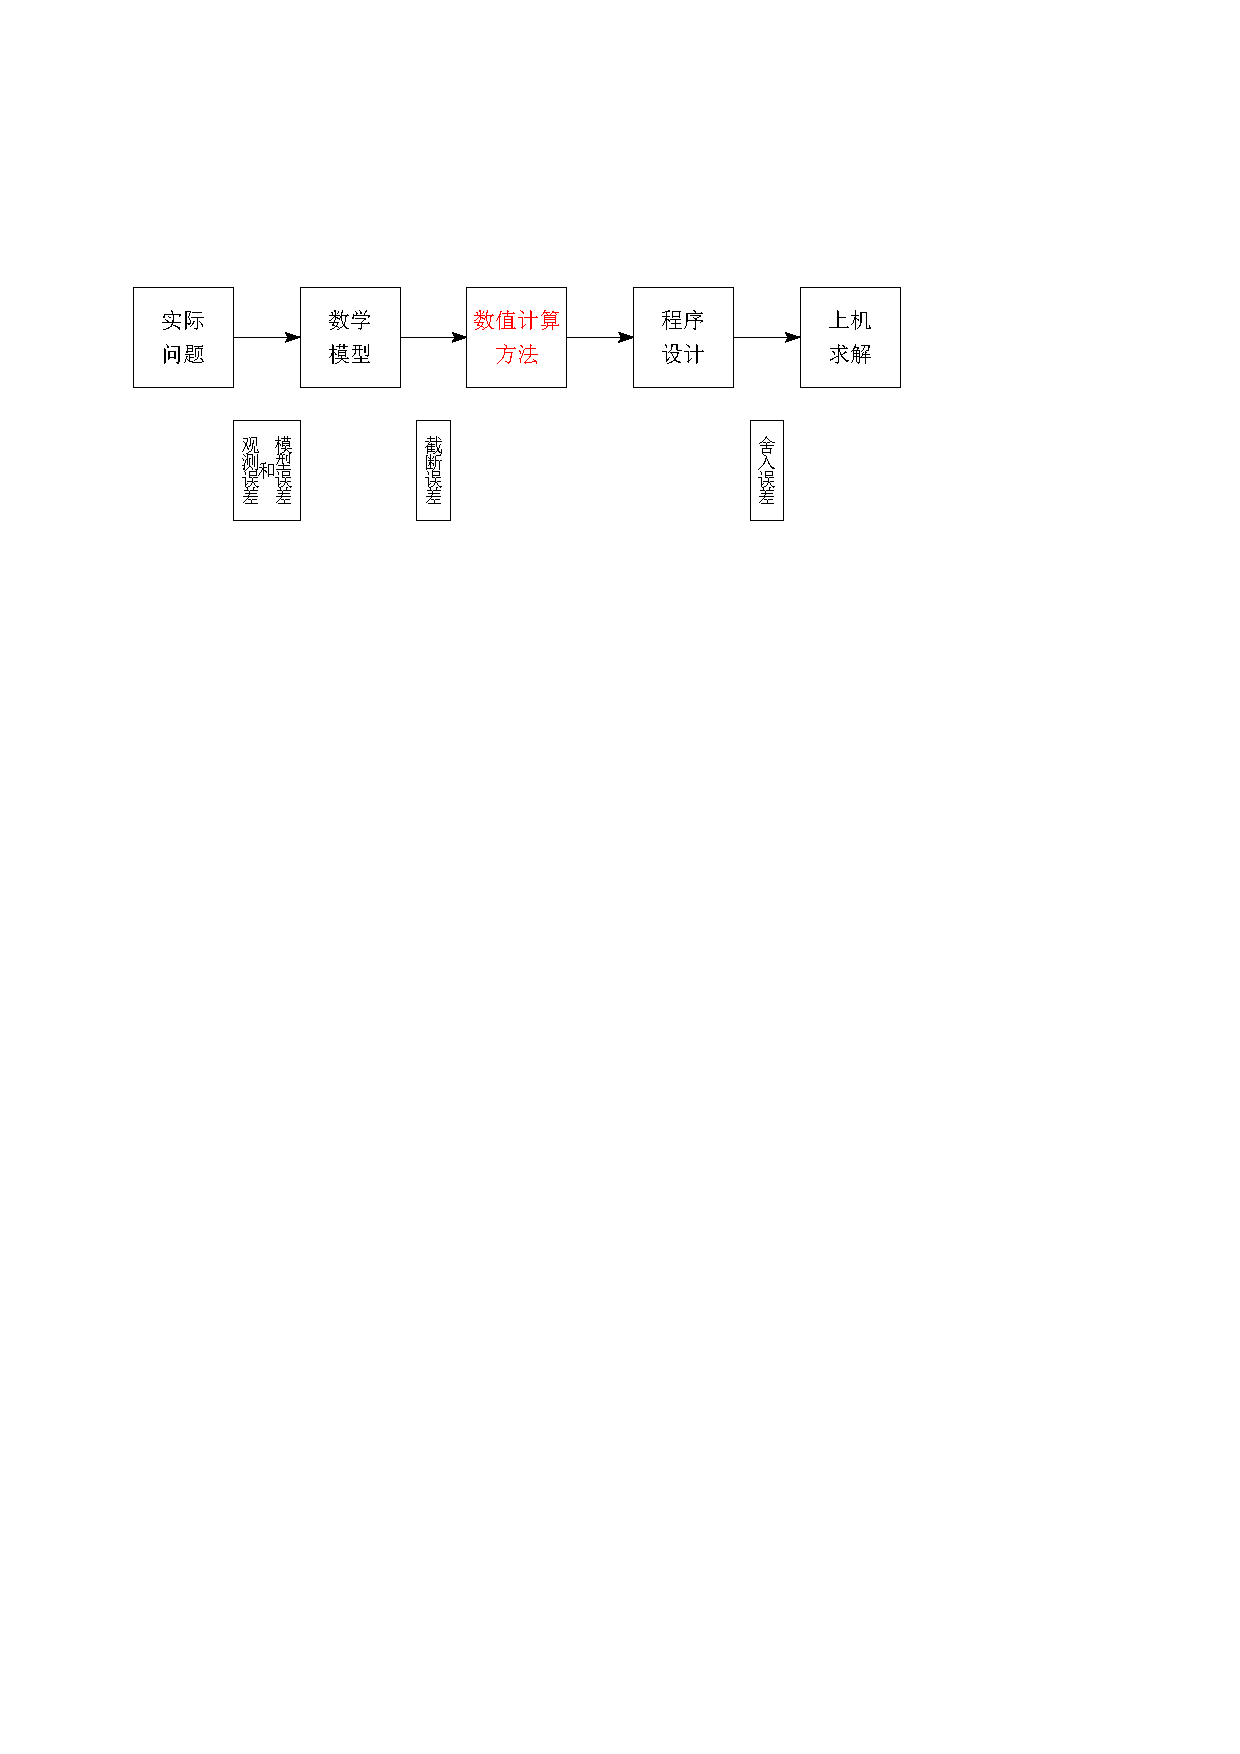
\includegraphics{image/误差.pdf}
\end{figure}
\subsection{误差度量}
\begin{definition}[误差]
    设$x$为精确值(准确值),$x^*$是$x$的一个近似值,称$e^* = x^*-x$为近似$x$的绝对误差或误差。
\end{definition}
\begin{definition}[误差限]
    如果精确值$x$与近似值$x^*$的误差的绝对值不超过某正数$\varepsilon$,即
    \[
        |e| = |x^*-x|<\varepsilon
    \]
    称$\varepsilon$为绝对误差限或误差限。
\end{definition}
\begin{definition}[相对误差]
    设$x$为精确值(准确值),$x^*$是$x$的一个近似值,称$\colorbox{yellow!50}{$r = \dfrac{e^*}{x^*}=\dfrac{x^*-x}{x^*}$}$为近似$x$的相对误差。
\end{definition}
\begin{definition}[相对误差限]
    如果有正数$\varepsilon_r$,使得$r = \left| \dfrac{e^*}{x^*} \right|<\varepsilon_r$,则称$\varepsilon_r$为$x$的相对误差限。
\end{definition}

\begin{definition}[有效数字]
    当$x$的误差限为\colorbox{yellow!50}{某一位}的半个单位,则\colorbox{yellow!50}{这一位}到第一个非零位的位数称为$x$的有效位数。若有效数字共有$n$个,则称$x$有$n$位有效数字,或者说$x$精确到$n$位。
    
    或者说对于用标准形式表示的近似值$x^*$
    \[
        \begin{array}{c}
            x^* = \pm 10^m\times \left( a_1+a_2\times 10^{-1}+\cdots+a_n\times 10^{-(n-1)} \right)\\
            a_{i}\in\left\{ 1,2,\cdots 9 \right\},\,i = 1,2,\cdots n-1
        \end{array}
    \]
    有
    \[
        |x^*-x|< \dfrac{1}{2}\times 10^{m-n+1}
    \]
\end{definition}
\begin{theorem}
    对于用标准形式表示的近似值$x^*$
    \[
        \begin{array}{c}
            x^* = \pm 10^m\times \left( a_1+a_2\times 10^{-1}+\cdots+a_n\times 10^{-(n-1)} \right)\\
            a_{i}\in\left\{ 1,2,\cdots 9 \right\},\,i = 1,2,\cdots n-1
        \end{array}
    \]
    若$x^*$具有$n$位有效数字,则其相对误差限为
    \[
        r\leqslant \dfrac{1}{2a_1}\times 10^{-(n-1)}
    \]
    反之,若$x^*$的相对误差限$r\leqslant \dfrac{1}{2(a_1+1)}\times 10^{-(n-1)}$,则$x^*$至少具有$n$位有效数字。
\end{theorem}
\begin{proof}
    对于$x^*$有
    \[
        a_1\times 10^{m} \leqslant|x^*|\leqslant(a_1+1)\times 10^{m}  
    \]
    则,相对误差限$r$
    \[
        r = \dfrac{|x^*-x|}{|x^*|} \leqslant \dfrac{\dfrac{1}{2}\times 10^{m-n+1}}{a_1\times 10^{m}} = \dfrac{1}{2a_1}\times 10^{-(n-1)}
    \]
    反之,若$r\leqslant \dfrac{1}{2(a_1+1)}\times 10^{-(n-1)}$,有
    \[
        |x^*-x| = r|x^*|<\dfrac{1}{2(a_1+1)}\times 10^{-(n-1)}\times (a_1+1)\times 10^{m} = \dfrac{1}{2}\times 10^{m-n+1}
    \]
    则$x^*$至少具有$n$位有效数字。证毕!
\end{proof}
\begin{theorem}
    四舍五入所得皆为有效数字。
\end{theorem}
\begin{proof}
    若将精确值$x$表示为
    \[
        x = \pm 10^m\times \left( a_1+a_2\times 10^{-1}+\cdots+a_n\times 10^{-(n-1)}+a_{n+1}\times 10^{-n}+\cdots \right)
    \]
    将$x$四舍五入到第$n$位得到$x^*$
    \[
        x^* = \pm 10^m\times \left( a_1+a_2\times 10^{-1}+\cdots+a_n^{\prime}\times 10^{-(n-1)} \right)
    \]
    对于四舍五入到第$n$位得到的$x^*$,有以下两种情况:
    \begin{enumerate}
        \item $a_n^{\prime}-a_n = 0,\ a_{n+1}<5$(靠近原点)
        \[
            \left| (a_n^{\prime}-a_n) - a_{n-1}\times 10^{-1} \right|<\dfrac{1}{2}
        \]
        \item $a_n^{\prime}-a_n = 1,\ 5\leqslant a_{n+1}<10$(远离原点)
        \[
            \left| (a_n^{\prime}-a_n) - a_{n-1}\times 10^{-1} \right|<\dfrac{1}{2}
        \]
    \end{enumerate}
    那么$|x^*-x|$有
    \[
        \begin{array}{ll}
            |x^*-x| &= 10^{m-n+1}\times \left| (a_n-a_n^{\prime}) + a_{n-1}\times 10^{-1} \right|\\
            &<\dfrac{1}{2}\times 10^{m-n+1}
        \end{array} 
    \]证毕!
\end{proof}
\begin{note}
    误差的传播:记$x^*$和$y^*$分别为$x$和$y$的近似值,则初始误差与计算结果中产生的误差有下列关系
    \[
        \varepsilon_{x^*\pm y^*} = \varepsilon_{x^*}+\varepsilon_{y^*},\ \varepsilon_{r_{x^*\pm y^*}} = \dfrac{\varepsilon_{x^*}+\varepsilon_{y^*}}{x^{*}\pm y^{*}}
    \]
    \[
        \varepsilon_{x^*\cdot y^*} = x^*\varepsilon_{y^*}+y^*\varepsilon_{x^*},\ \varepsilon_{r_{x^*\cdot y^*}} = \dfrac{x^*\varepsilon_{y^*}+y^*\varepsilon_{x^*}}{x^{*}\cdot y^{*}}
    \]
    \[
        \varepsilon_{\frac{x^*}{y^*}} \approx \dfrac{x^*\varepsilon_{y^*}+y^*\varepsilon_{x^*}}{y^{*2}},\ \varepsilon_{r_{\frac{x^*}{y^*}}} \approx \dfrac{x^*\varepsilon_{y^*}+y^*\varepsilon_{x^*}}{x^{*}\cdot y^{*}}
    \]
    \[
        \begin{array}{c}
            \varepsilon(f(\boldsymbol{x}^*))\approx \sum\limits_{i = 1}^{n}\left|\dfrac{\partial f(\boldsymbol{x}^*)}{\partial x_i}\right|\varepsilon(x_i^*)\\
            \varepsilon_r(f(\boldsymbol{x}^*))\approx \sum\limits_{i = 1}^{n}\left|\dfrac{\partial f(\boldsymbol{x}^*)}{\partial x_i}\right|\dfrac{\varepsilon(x_i^*)}{f(\boldsymbol{x}^*)}
        \end{array}
    \]
\end{note}
\begin{example}
    设$V = \dfrac{4\pi R^3}{3}$,当半径$R$有误差时,求球体积$V$的相对误差与$R$的相对误差的关系。\Stars{3.5}{}
    \[
        e_r[V] = \dfrac{e[V]}{V} = \dfrac{4\pi R^2\cdot e[R]}{\dfrac{4\pi R^3}{3}} = 3\dfrac{e[R]}{R} = 3e_r{R}
    \]
\end{example}
\begin{example}
    设$x>0$,$x$的相对误差为$\delta$,求$\ln x$的误差。\Stars{4}{}
    \[
        \ln x-\ln x^* = \ln \dfrac{x}{x^*} = \ln \dfrac{x-x^*+x^*}{x^*} = \ln (\delta+1)\approx \delta
    \]
    或者
    \[
        e(\ln x^*) \approx \dfrac{e(x^*)}{x^*} = e_r(x^*) = \delta
    \]
\end{example}
\begin{example}
    设$x$的相对误差为$2\%$,求$x^n$的相对误差。\Stars{4}{}
    \[
        e_r(x^n)\approx n\dfrac{x^{*(n-1)}e(x^*)}{x^{*(n)}} = ne_r(x^*) = 0.02n
    \]
\end{example}

\subsection{误差分析方法与原则}
\begin{definition}[病态问题]
    对于一个数值问题,若输入数据的微小扰动(即误差)会引起输出数据(即问题解)相对误差很大,这就是\textcolor{red!50}{病态问题}。
\end{definition}
\begin{definition}[数值稳定性]
    一个算法如果原始数据有扰动(即误差),二计算过程中舍入误差不增长,则称此算法是数值稳定的;否则,若误差增长则称算法数值不稳定。
\end{definition}
\begin{note}
    数值运算中误差分析的方法与原则
    \begin{itemize}
        \item 避免除数的绝对值远远小于被除数
        \item 避免两相近数相减
        \item 防止大数“吃掉”小数
        \item 注意简化计算步骤,减少运算次数
    \end{itemize}
\end{note}